\subsubsection{UC3 - Registrazione}
\begin{figure}[H]
	\centering
	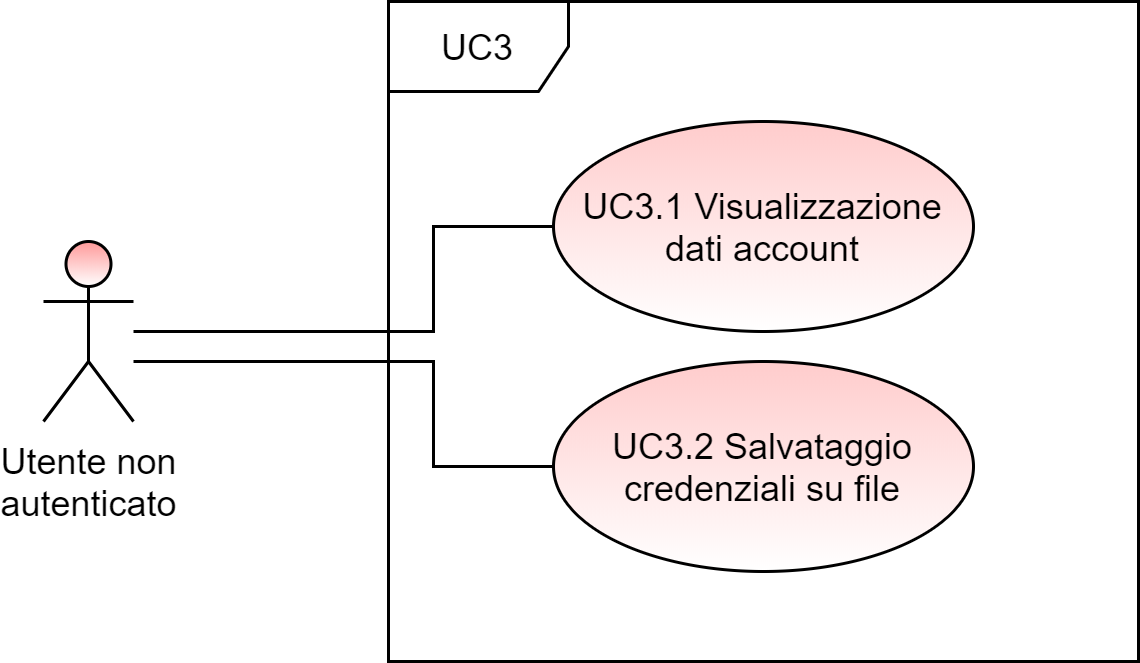
\includegraphics[scale=\ucs]{./res/img/UC3.png}
	\caption {UC3 - Registrazione}
\end{figure}
\begin{itemize}
	\item \textbf{Attori primari:} \una{};
	\item \textbf{Attori secondari:} \re{};
	\item \textbf{Descrizione:} dopo aver richiesto la creazione di un nuovo account Ethereum\ped{\textit{G}} tramite l’utilizzo del comando \signup{}, l’utente visualizza a video le credenziali del nuovo account creato; Tali credenziali includono:
	\begin{itemize}
		\item address: indirizzo del nuovo account creato;
		\item private key\ped{\textit{G}}: chiave privata utilizzata per accedere alla rete Ethereum;
		\item mnemonic phrase\ped{\textit{G}}: frase composta da 12 parole, utilizzata per generare la chiave privata o per eseguire il login.
	\end{itemize}
	\item \textbf{Scenario principale:}
	\begin{itemize}
		\item l’utente richiede la creazione di un account all’interno della rete Ethereum\ped{\textit{G}} mediante il comando \signup{};
		\item vengono visualizzate le credenziali del nuovo account creato. 
	\end{itemize}
	\item \textbf{Precondizione:} l'utente vuole creare un nuovo account; 
	\item \textbf{Postcondizione:} l’account è stato creato correttamente. 
\end{itemize}